%to have line numbers
%\RequirePackage{lineno}
\documentclass[10pt, letterpaper]{article}      
\usepackage[margin=.1cm,font=small,labelfont=bf]{caption}[2007/03/09]
%\usepackage{endnotes}
%\let\footnote=\endnote
\usepackage{setspace}
\usepackage{longtable}                        
\usepackage{anysize}                          
\usepackage{natbib}                           
%\bibpunct{(}{)}{,}{a}{,}{,}                   
\bibpunct{(}{)}{,}{a}{}{,}                   
\usepackage{amsmath}
\usepackage[% draft,
pdftex]{graphicx} %draft is a way to exclude figures                
\usepackage{epstopdf}
\usepackage{hyperref}                             % For creating hyperlinks in cross references
\hypersetup{pdfborder={0 0 0.4}} %have nice light boxes on refs

% \usepackage[margins]{trackchanges}

% \note[editor]{The note}
% \annote[editor]{Text to annotate}{The note}
%    \add[editor]{Text to add}
% \remove[editor]{Text to remove}
% \change[editor]{Text to remove}{Text to add}

%TODO make it more standard before submission: \marginsize{2cm}{2cm}{1cm}{1cm}
\marginsize{1cm}{1cm}{.5cm}{.5cm}%{left}{right}{top}{bottom}   
					          % Helps LaTeX put figures where YOU want
 \renewcommand{\topfraction}{1}	                  % 90% of page top can be a float
 \renewcommand{\bottomfraction}{1}	          % 90% of page bottom can be a float
 \renewcommand{\textfraction}{0.0}	          % only 10% of page must to be text

 \usepackage{float}                               %latex will not complain to include float after float

\usepackage[table]{xcolor}                        %for table shading
\definecolor{gray90}{gray}{0.90}
\definecolor{orange}{RGB}{255,128,0}

\renewcommand\arraystretch{.9}                    %for spacing of arrays like tabular

%-------------------- my commands -----------------------------------------
\newenvironment{ig}[1]{
\begin{center}
 %\includegraphics[height=5.0in]{#1} 
 \includegraphics[height=3.3in]{#1} 
\end{center}}

 \newcommand{\cc}[1]{
\hspace{-.13in}$\bullet$\marginpar{\begin{spacing}{.6}\begin{footnotesize}\color{blue}{#1}\end{footnotesize}\end{spacing}}
\hspace{-.13in} }

%-------------------- END my commands -----------------------------------------



%-------------------- extra options -----------------------------------------

%%%%%%%%%%%%%
% footnotes %
%%%%%%%%%%%%%

%\long\def\symbolfootnote[#1]#2{\begingroup% %these can be used to make footnote  nonnumeric asterick, dagger etc
%\def\thefootnote{\fnsymbol{footnote}}\footnote[#1]{#2}\endgroup}	%see: http://help-csli.stanford.edu/tex/latex-footnotes.shtml

%%%%%%%%%%%
% spacing %
%%%%%%%%%%%

% \abovecaptionskip: space above caption
% \belowcaptionskip: space below caption
%\oddsidemargin 0cm
%\evensidemargin 0cm

%%%%%%%%%
% style %
%%%%%%%%%

%\pagestyle{myheadings}         % Option to put page headers
                               % Needed \documentclass[a4paper,twoside]{article}
%\markboth{{\small\it Politics and Life Satisfaction }}
%{{\small\it Adam Okulicz-Kozaryn} }

%\headsep 1.5cm
% \pagestyle{empty}			% no page numbers
% \parindent  15.mm			% indent paragraph by this much
% \parskip     2.mm			% space between paragraphs
% \mathindent 20.mm			% indent math equations by this much

%%%%%%%%%%%%%%%%%%
% extra packages %
%%%%%%%%%%%%%%%%%%

\usepackage{datetime}


\usepackage[latin1]{inputenc}
\usepackage{tikz}
\usetikzlibrary{shapes,arrows,backgrounds}


%\usepackage{color}					% For creating coloured text and background
%\usepackage{float}
\usepackage{subfig}                                     % for combined figures

\renewcommand{\ss}[1]{{\colorbox{blue}{\bf \color{white}{#1}}}}
\newcommand{\ee}[1]{\endnote{\vspace{-.10in}\begin{spacing}{1.0}{\normalsize #1}\end{spacing}\vspace{.20in}}}
\newcommand{\emd}[1]{\ExecuteMetaData[/tmp/tex]{#1}} % grab numbers  from stata

%TODO before submitting comment this out to get 'regular fornt'
\usepackage{sectsty}
\allsectionsfont{\normalfont\sffamily}
\usepackage{sectsty}
\allsectionsfont{\normalfont\sffamily}
\renewcommand\familydefault{\sfdefault}

%\usepackage[margins]{trackchanges}
\usepackage{rotating}
\usepackage{catchfilebetweentags}

\usepackage{abstract}
\renewcommand{\abstractname}{}    % clear the title
\renewcommand{\absnamepos}{empty} % originally center
%-------------------- END extra options -----------------------------------------
\date{{}\today \hspace{.2in}\xxivtime}
\title{  % remember to have Vistula University!!
  Covid19 and Urban Unhappiness
}
\author{
Adam Okulicz-Kozaryn\thanks{EMAIL: adam.okulicz.kozaryn@gmail.com
  \hfill I thank XXX.  All mistakes are mine.} \\
{\small Rutgers - Camden  % and Vistula University
}
}

\begin{document}

%%\setpagewiselinenumbers
%\modulolinenumbers[1]
%\linenumbers

\bibliographystyle{/home/aok/papers/root/tex/ecta}
\maketitle
\vspace{-.4in}
\begin{center}

\end{center}


\begin{abstract}
  \noindent  We find life satisisfaction to
  decrease in cities v smaller areas post-pandemic in United Kingdom, 
 the Netherlands, and Uruguay. 
  % 
  Whats remarkable is a large differential or effect sizes pre-post
  pandemic for cities v smaller areas.  Cities  v smaller areas became 2x less happy
 post-pandemic v pre-pandemic. To be precise, there has been 2x decrease for
 United Kingdom and  the Netherlands.  For Uruguay there has been an increase in
 life satisfaction across both cities and smaller places, but the increase has
 been 2x smaller for cities v smaller areas. In relative terms, effect size differentials are remerkable--it is rare to see in SWB research 2x or 200\% differentials. In
 absolute terms, effect sizes are large, too. While .2-.25 difference on 1-10
 SWB scale is small, one must take into account massive scale of
 urbanization--.2-.25 decrease on 1-10 SWB scale applied to millions of people
 is a massive slump in human development. Findings are correlational, not causal. 
\end{abstract}
\vspace{.15in} 
\noindent{\sc urban, rural, urban-rural happienss gradient, happiness,
  subjective wellbeing
}
\vspace{.25in} 

\begin{spacing}{1.4} %TODO MAYBE before submission can make it like 2.0
\rowcolors{1}{white}{gray90}

%  instead \ExecuteMetaData[../out/tex]{ginipov} do \emd{ginipov}

% \begin{figure}[H]
%  \includegraphics[height=3in]{../out/gov_res_trust.pdf}\centering\label{gov_res_trust}
% \caption{woo}
% \end{figure}


%TODO !!!! have input here aok_var_des



% %table centered on decimal points:)
% \begin{table}[H]\centering\footnotesize
% \caption{\label{freq_im_god} importance of God}
% \begin{tabular} {@{} lrrrr @{}}   \hline 
% Item& Number & Per cent   \\ \hline
% 1(not at all)&    9,285&  9\\
% 2&    3,555&        3\\
% 3&    3,937&        4\\
% 4&    2,888&        3\\
% 5&    7,519&        7\\
% 6&    5,175&        5\\
% 7&    6,050&        6\\
% 8&    8,067&        8\\
% 9&    8,463&        8\\
% 10&   52,385&       49\\
% Total&  107,324&      100\\ \hline
% \end{tabular}\end{table}


% % Define block styles
% \tikzstyle{block} = [rectangle, draw, fill=black!20, 
%     text width=10em, text centered, rounded corners, minimum height=4em]
% \tikzstyle{b} = [rectangle, draw,  
%     text width=6em, text centered, rounded corners, minimum height=4em]
% \tikzstyle{line} = [draw, -latex']
% \tikzstyle{cloud} = [draw, ellipse,fill=black!20, node distance = 5cm,
%     minimum height=2em]
    
% \begin{tikzpicture}[node distance = 2cm, auto]
%     % Place nodes
%     \node [block] (lib) {liberalism, egalitarianism, welfare};
%     \node [block, below of=lib] (con) {conservatism, competition, individualism};
%     \node [cloud, right of=con] (ls) {well-being};
%     \node [block, below of=ls] (cul) {genes, culture};
%     \node [b, left of =lib, node distance = 4cm] (c) {country-level};
%     \node [b, left of =con,  node distance = 4cm] (c) {person-level};
%     % Draw edges
%     \path [line] (lib) -- (ls);
%     \path [line] (con) -- (ls);
%     \path [line,dashed] (cul) -- (ls);
% \end{tikzpicture}


%PUT THIS NOTE, polish and put to /root/author_what_data --ALWAYS
%stick here stuff as i run it!!! maybe comment out later...

'Here is the great city: here have you nothing to seek and everything to lose.' Nietzsche\\


Covid19 has changed our way of life. Indeed, changes seem persistent
  to large degree and there seems to be no coming back. One of the key areas
  affected is urbanism. Pre-pandemic there has been city renewal, rebirth, and indeed
  triumphalism. Post-pandemic there is urban scepticism, scare, and indeed, in
  some cases, collapse.


Timing is everything. Ed Glaeser wrote a bestselling book 'Triumph of the city'
just several years before the collapse of the city. Cities are hollowed out by
the covid19 pandemic.

% Celebrity urbanlogy \citep{peck16} does not take into account inherently urban
% disadvantages such as higher crime or infectious disease spread. What is missed
% is that crime disease are urban feature--they are higher per capita in cities
% because city itself increases them. These are universal laws, like physics laws,
% and they are best illustrated with a graph

We know that one of the disadvantages of city is increased infectious disease
spread. Put simply, one city feature is increased
infectious disease spread. Indeed such population scaling is so consistent and
strong, it is universal\citep{blissCL_nov4_14,bettencourt10,bettencourt10b,bettencourt07}. Indeed, it could be called ``law'', like physics laws such as gravity.

Covid19, an infectious disease, fits this pattern  \citep{stier2021early}. 

Massive infectious diseases happene every now and then, SARS, Ebola, etc, and recently COVID19. The
research hypothesis is that as cities suffer disporportionately from infectious
diseases, city happiness decreased disproportionaly as well with covid19.


   %

  In present study we take a human development perspective using a measure of
  human flourishinng, subjective wellbeing (swb).
  Boilerplate from sen stiglitz and UN!! (see slides from cSWB).

  
\section{Data}

We use World Values Survey cumulative file 1981-2022, 7 wave file. We proceed as
follows with the sample selection. Covid19 didn't really take off untill later
in 2020, peaked in 2021, and still had a considerable effect in 2022. Hence we
look at data in 2021 and 2022. Data in 2021 has only developing countries, and
rather small with small cities: Armenia, Kenya, Maldives, Morocco, and
Venezuela. Hence, we will focus on 2022: Czechia, Libya, Netherlands, Northern
Ireland, Slovakia, United Kingdom, and Uruguay. Next, we check sample sizes by
year and urbanicity (X049) for each country. We exclude:  Czechia: no city >500k
before 2022. Libya: only 7 respondents in city >500k before 2022. Northern
Ireland: total sample size is 447 and only one wave. Slovakia: only 61
respondents in city >500k pre 2022. Which leavs us with United Kingdom (GBR),
Netherlands (NLD), and Uruguay (URY).

\section{Results}

\begin{figure}[H]
 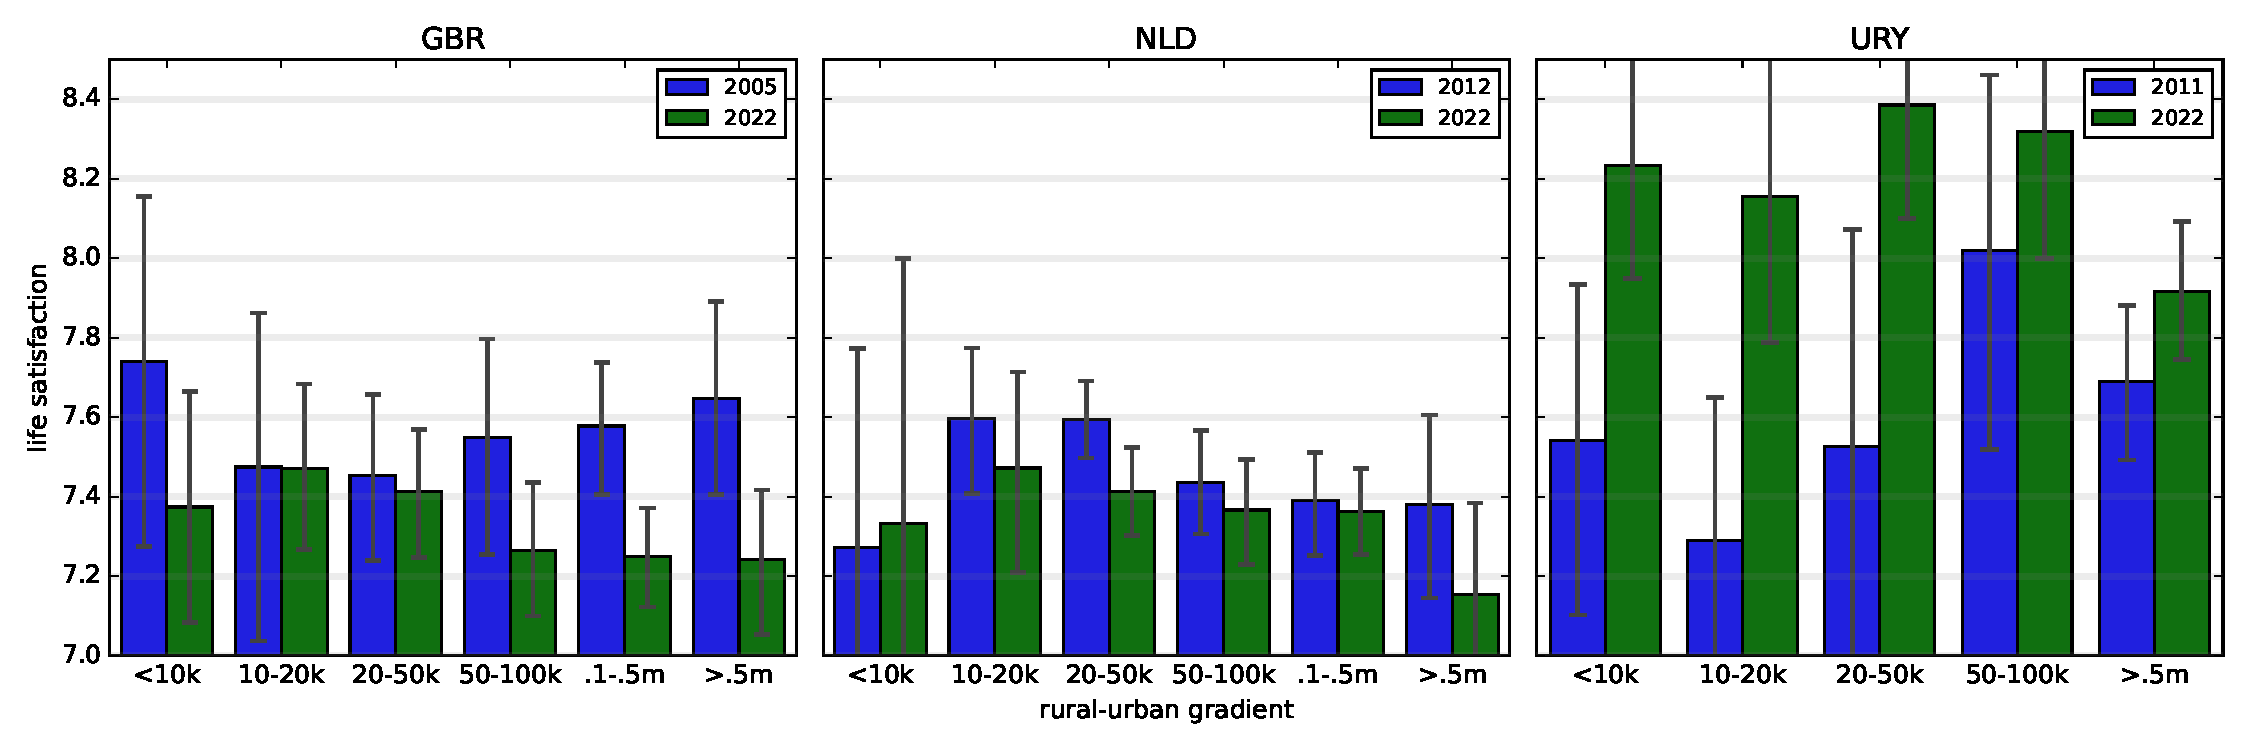
\includegraphics[width=7in]{bar.pdf}\centering\label{bar}
\caption{Life satisfaction ($1=unhappy$ to $10=happy$) means with 95\% CI against rural urban gradient categories. $GBR=$ United Kingdom, $NLD=$ Netherlands, $URY=$ Uruguay. Note: URY is missing .1-.5m cat due to small cell sizes.}
 \end{figure}


GBR: so prepandemic -10k happiest; pandemic: both smallest and largest most hit; unexpected for smallest, what it could be?

may be some country specific


NLD: rural not much change pre post, except for largest cities as expected; but also weirdly 10-20, and esp 20-50


URY is a different story: SWB increased everywhere ; and increased in >500k too, but increased least there--so also as expected

Many of the CI are wide. Next we test the differences with regression. First,
since the focus is on cities v smaller areas (rural and towns), for simplicity,
we collapse categories upto .5m into one as rural and towns and contrast this
category with cities (larger than .5m). 


The hypothesis is that while the pandemic decreased wellbeing in general, it
especially did so in the cities. Again, a city feature is increased
infectious disease spread.

Hence, what we are really focused on here is  the big city difference v the
smaller areas. Another 2 reasons are technical--it is simpler exposition to have
urban dichotomy as opposed to full gradient, given that we also have 2 other
breakdowns: pre-post covid and by country. Last but not least, cell sizes run
small with too many breakdowns of this small dataset. Future research, when more
data become available may test full gradient.  


We break up our analyses by country and then within each country by rural and
towns (<.5m) v cities (>.5m). We regress life satisfaction on 2022 dummy, base
case being latest pre-pandemic wave as shown in fig \ref{bar}. 
% First we could look at overall change in happiness pre-post pandemic or such
% change for all areas except large cities.
 Bivariate regression results are set in table \ref{a}.
 Effect sizes on 2022 dummy replicate findings from fig \ref{bar}. For GBR the
 difference pre-post panemic is about .2 for rural areas and towns (<.5m), and
 the difference for cities (>.5m) is about .4, and so forth for NLD and URY.
 %
 Whats remarkable is about 2x difference for GBR and NLD and 3x for URY, this is
 a very strong differential. Cities v smaller areas became 2x to 3x less happy
 post-pandemic v pre-pandemic. 
 Still one of the coef for NLD not sig, and weakly
sig for URY, and there is left out variable bias.\footnote{diffs should be even
  bigger controlling for swb predictors! urban rural happiness gradient often
  emerges only after contrilling for swb predictors \citep{aok21}.} Hence,  we elaborate models with an
extensive set of SWB predictors in table \ref{b}.
 
 
\begin{spacing}{.9} \begin{table}[H]\centering   \begin{scriptsize} \begin{tabular}{p{1.8in}p{.5in}p{.5in}|p{.5in}p{.5in}|p{.5in}p{.5in}|p{.5in}p{.5in}p{.5in}p{.5 in}p{.5in}p{.5 in}}\hline&\multicolumn{2}{c}{GBR}&\multicolumn{2}{c}{NLD}&\multicolumn{2}{c}{URY}\\                     &   $<.5m$   &     $>.5m$   &   $<.5m$   &     $>.5m$   &   URYrurTow   &     URYcity   \\
2022                &       -0.21** &       -0.41** &       -0.12** &       -0.23   &        0.75***&        0.23+  \\
constant            &        7.54***&        7.65***&        7.50***&        7.38***&        7.54***&        7.69***\\
N                   &        3111   &         521   &        3572   &         373   &        1154   &         836   \\
 \hline + 0.10 * 0.05 ** 0.01 *** 0.001; robust std err \end{tabular}\end{scriptsize}\caption{\label{a}OLS regressions of life satisfaction.}\end{table} \end{spacing}


\begin{spacing}{.9} \begin{table}[H]\centering   \begin{scriptsize} \begin{tabular}{p{1.8in}p{.5in}p{.5in}|p{.5in}p{.5in}|p{.5in}p{.5in}|p{.5in}p{.5in}p{.5in}p{.5 in}p{.5in}p{.5 in}}\hline\hline&\multicolumn{2}{c}{GBR}&\multicolumn{2}{c}{NLD}&\multicolumn{2}{c}{URY}\\                     &   $<.5m$   &     $>.5m$   &   $<.5m$   &     $>.5m$   &   URYrurTow   &     URYcity   \\
2022                &       -0.18*  &       -0.39+  &       -0.20***&       -0.45** &        0.42***&        0.21   \\
income              &        0.09***&        0.01   &        0.06***&        0.14***&        0.07*  &        0.13***\\
age                 &       -0.03*  &       -0.08** &       -0.02+  &       -0.06+  &        0.00   &       -0.06** \\
age2                &        0.00** &        0.00** &        0.00** &        0.00*  &       -0.00   &        0.00** \\
male                &       -0.18** &       -0.13   &       -0.11*  &       -0.27+  &        0.06   &        0.19   \\
married or living together as married&        0.53***&        0.74***&        0.44***&        0.23   &        0.46** &        0.06   \\
divorced/separated/widowed&        0.07   &        0.15   &       -0.11   &       -0.14   &       -0.37+  &       -0.19   \\
autonomy            &       -0.11*  &       -0.07   &       -0.11** &       -0.01   &       -0.06   &        0.06   \\
freedom             &        0.44***&        0.42***&        0.35***&        0.43***&        0.43***&        0.36***\\
trust               &        0.12+  &        0.42** &        0.43***&        0.28+  &       -0.05   &        0.10   \\
postmaterialist     &       -0.05   &       -0.18   &       -0.11*  &        0.14   &       -0.02   &        0.15   \\
god important       &        0.01   &        0.05*  &        0.02*  &       -0.01   &        0.05** &        0.06** \\
constant            &        4.08***&        5.95***&        4.59***&        4.80***&        3.47***&        4.58***\\
N                   &        1985   &         309   &        2283   &         237   &         736   &         579   \\
 \hline + 0.10 * 0.05 ** 0.01 *** 0.001; robust std err \end{tabular}\end{scriptsize}\caption{\label{b}OLS regressions of life satisfaction.}\end{table} \end{spacing}

Again about 2x difference for GBR and NLD persists, and for URY it is reduced
from about 3x to about 2x as well

Finally, as a robustness check we add health variable in table
\ref{c}. Obviously, there will bethen confounding between pre-post covid and
health by definition. 
And there will be also confounding between urbanicity and health as again covid
is more prevelent in cities.  Hence these regressions are less useful in determing pre-post
covid urb-rur differentials. Now taking into account health, as expected,
results on over time difference are smaller and less significant (pre-post
confounding with health). Remarkably though, the urbanicity differentials even
though less statistically significant are still about x2 for GBR and URY and
even stronger for NLD. Perhaps and arguably covid city in addition to bad health
caused other problems such as misanthrophy and overal malaise. Future research
is needed. 

\begin{spacing}{.9} \begin{table}[H]\centering   \begin{scriptsize} \begin{tabular}{p{1.8in}p{.5in}p{.5in}|p{.5in}p{.5in}|p{.5in}p{.5in}|p{.5in}p{.5in}p{.5in}p{.5 in}p{.5in}p{.5 in}}\hline\hline&\multicolumn{2}{c}{GBR}&\multicolumn{2}{c}{NLD}&\multicolumn{2}{c}{URY}\\                     &   $<.5m$   &     $>.5m$   &   $<.5m$   &     $>.5m$   &   URYrurTow   &     URYcity   \\
2022                &       -0.12   &       -0.26   &       -0.06   &       -0.24+  &        0.44***&        0.23   \\
health              &        0.48***&        0.67***&        0.62***&        0.77***&        0.56***&        0.32** \\
income              &        0.05** &       -0.01   &        0.04***&        0.08** &        0.05   &        0.12***\\
age                 &       -0.02*  &       -0.07*  &       -0.01   &       -0.03   &        0.01   &       -0.05*  \\
age2                &        0.00** &        0.00** &        0.00** &        0.00+  &       -0.00   &        0.00*  \\
male                &       -0.16*  &       -0.15   &       -0.09+  &       -0.23+  &       -0.01   &        0.14   \\
married or living together as married&        0.49***&        0.60** &        0.38***&        0.21   &        0.41** &        0.04   \\
divorced/separated/widowed&        0.05   &        0.20   &       -0.15   &       -0.27   &       -0.36+  &       -0.16   \\
autonomy            &       -0.12** &       -0.09   &       -0.10** &        0.07   &       -0.09   &        0.04   \\
freedom             &        0.38***&        0.29***&        0.29***&        0.31***&        0.40***&        0.35***\\
trust               &        0.07   &        0.28*  &        0.34***&        0.21   &       -0.07   &        0.01   \\
postmaterialist     &       -0.05   &       -0.26+  &       -0.09*  &        0.06   &        0.01   &        0.12   \\
god important       &        0.01   &        0.02   &        0.02+  &        0.00   &        0.05** &        0.06** \\
constant            &        2.72***&        4.29***&        2.46***&        2.01*  &        1.31+  &        3.31***\\
N                   &        1985   &         309   &        2279   &         236   &         736   &         578   \\
 \hline + 0.10 * 0.05 ** 0.01 *** 0.001; robust std err \end{tabular}\end{scriptsize}\caption{\label{c}OLS regressions of life satisfaction.}\end{table} \end{spacing}

Our final set of results will pool all the data together. Earlier we split the
sample by pre-post and large city v town and rural for simplicity and ease of
interpretation, but it is also useful to formally test the differences with
interactions. 

in table \ref{d} we start with a basic model where we regress life satisfaction
on a dummy for largest cities and post-pandemic wave dummy $=1 if yr==2022$, we
also include country dummies as we now pull all the data together. Finally, we
also include year dummies in addition to pre-post dummy as data were collected
in different countries in differemt years.

in column a1, as expected we see that post pandemic swb went down by .2, and
especially so for cities  by additional .26. addition of basic controls in a2,
post*city interaction stays about the same. extended controls in a3, same. only
addition of hea in a4 cuts it to .21, and addition of freedom in a5 cuts most
substaintally to .15 an kills significance. freedom kills it! future research: look more at freedom

\begin{spacing}{.9} \begin{table}[H]\centering   \begin{scriptsize} \begin{tabular}{p{1.8in}p{.5in}p{.5in}p{.5in}p{.5in}p{.5in}p{.5in}p{.5in}p{.5in}p{.5in}p{.5 in}p{.5in}p{.5 in}}\hline                     &          a1   &          a2   &          a3   &          a4   &          a5   \\
post pandemic            &       -0.20** &       -0.13+  &       -0.10   &       -0.02   &       -0.18*  \\
city lg500k&        0.05   &        0.19*  &        0.20*  &        0.11   &        0.07   \\
post pandemic $\times$ city lg500k&       -0.26*  &       -0.26*  &       -0.26*  &       -0.21+  &       -0.15   \\
United Kingdom      &       -0.04   &        0.03   &        0.08   &       -0.01   &       -0.04   \\
Uruguay             &        0.82***&        0.92***&        0.95***&        0.68***&        0.43***\\
2011                &       -0.82***&       -0.72***&       -0.54***&       -0.47***&       -0.44***\\
2012                &       -0.10   &        0.15+  &        0.11   &        0.02   &        0.05   \\
income              &               &        0.14***&        0.13***&        0.08***&        0.08***\\
age                 &               &       -0.05***&       -0.04***&       -0.03***&       -0.03***\\
age2                &               &        0.00***&        0.00***&        0.00***&        0.00***\\
male                &               &       -0.16***&       -0.17***&       -0.16***&       -0.11** \\
married or living together as married&               &        0.46***&        0.46***&        0.39***&        0.44***\\
divorced/separated/widowed&               &        0.01   &        0.01   &       -0.03   &       -0.07   \\
god important       &               &               &        0.03***&        0.03***&        0.02***\\
trust               &               &               &        0.38***&        0.25***&        0.26***\\
postmaterialist     &               &               &       -0.04   &       -0.05+  &       -0.04   \\
autonomy            &               &               &       -0.10***&       -0.10***&       -0.09***\\
health              &               &               &               &        0.71***&               \\
freedom             &               &               &               &               &        0.40***\\
constant            &        7.58***&        7.42***&        7.14***&        4.40***&        4.47***\\
N                   &        9196   &        7746   &        6038   &        6032   &        5970   \\
 \hline + 0.10 * 0.05 ** 0.01 *** 0.001; robust std err \end{tabular}\end{scriptsize}\caption{\label{c}OLS regressions of life satisfaction.}\end{table} \end{spacing}

\section{conclusion and discussion}

actually before pandemic city happiness was on the rise relative to rur, at
least in the us--millenials paper that city swb was doing better v rur arguably
because rural has been left behind

FUTURE RESEARCH SEC:

Covid may be largely gone. And another massive pandemic may be decades ahead. But covid effects are likely to last for years to come, arguably including urban scare, and possibly an urban crisis. As time passes future research should retest the relationships. Also as more data becomes available it'd be instructive to zoom in on most affected societies such as Italy and the US--negative effects are likely to be greater there.



TODO: have separate som-r.tex as opposed to having it below; and in paper say
see supplemetary material as opposed to see appendix!

% \section*{\Huge ONLINE APPENDIX}
% \textbf{[note: this section will NOT be a part of the final version of
%   the manuscript, but will be available online instead]} %hence everything below
%                                 %is organized byu section, not subsection
% !!!
% have most of the stuff outputted to online appendix:)--start with that and then
% select stuff to paper--have brief narrative describng patterns in online app too
% !!!

% \section*{Variables' definitions, coding, and distributions}
% \label{app_var_des}


% %\input{/tmp/a.tex} %aok_var_des

% % \begin{spacing}{.9}
% %   \begin{table}[H]\centering \caption{Summary statistics.} \label{sumSta} \begin{scriptsize} \begin{tabular}{p{1.8in}p{.5in}p{.5in}p{.5in}p{.5in}p{.5in}p{.5in}p{.5in}p{.5in}p{.5in}p{.5
% %             in}p{.5in}p{.5 in}}\hline
% %         \input{/tmp/aha2.tex}
% %          \end{tabular}\end{scriptsize}\end{table}
% % \end{spacing}

% % \begin{spacing}{.9}
% %   \begin{table}[H]\centering \caption{Correlation matrix.} \label{sumSta} \begin{scriptsize} \begin{tabular}{@{}
% %           p{1.2in} rrrrrrrrrrrrr @{}}\hline
% %         \input{/tmp/ahb2.tex}\hline
% %          \end{tabular}\end{scriptsize}\end{table}
% % \end{spacing}



% Table XXX shows variable distributions. If a variable has more than
% 10 categories it is classified into bins...

% %\input .... %TODO !!!! have input here histograms

% \section*{Additional Descriptive Statistics}
% \label{app_des_sta}

% %make sure i have [H] or h! ???
% % \begin{table}[H]
% % \caption{}
% % \centering
% % \label{}
% % \begin{scriptsize}
% % \input{../out/reg_c.tex}
% % \end{scriptsize}
% % \end{table}

%\newpage
%\theendnotes
\bibliography{/home/aok/papers/root/tex/ebib.bib,covidCity.bib}

\end{spacing}
\end{document}
